\thispagestyle{duongvaotoanhocnone}
\pagestyle{duongvaotoanhoc}
\everymath{\color{duongvaotoanhoc}}
\graphicspath{{../duongvaotoanhoc/pic2/}}
\blfootnote{$^1$\color{duongvaotoanhoc}Bài viết gốc: {Infinity Category Theory Offers a Bird's--Eye View of Mathematics}, đăng trên {Scientific American}, Volume $325$, Issue $4$, October $2021$.}
\blfootnote{$^2$\color{duongvaotoanhoc}Johns Hopkins University, chuyên gia về lý thuyết phạm trù bậc cao và lý thuyết đồng luân, các công trình của cô liên quan đến phạm trù mô hình và nền tảng của lý thuyết phạm trù vô cực}
\blfootnote{$^3$\color{duongvaotoanhoc}Universit\'e Paris--Saclay.}
\begingroup
\AddToShipoutPicture*{\put(0,616){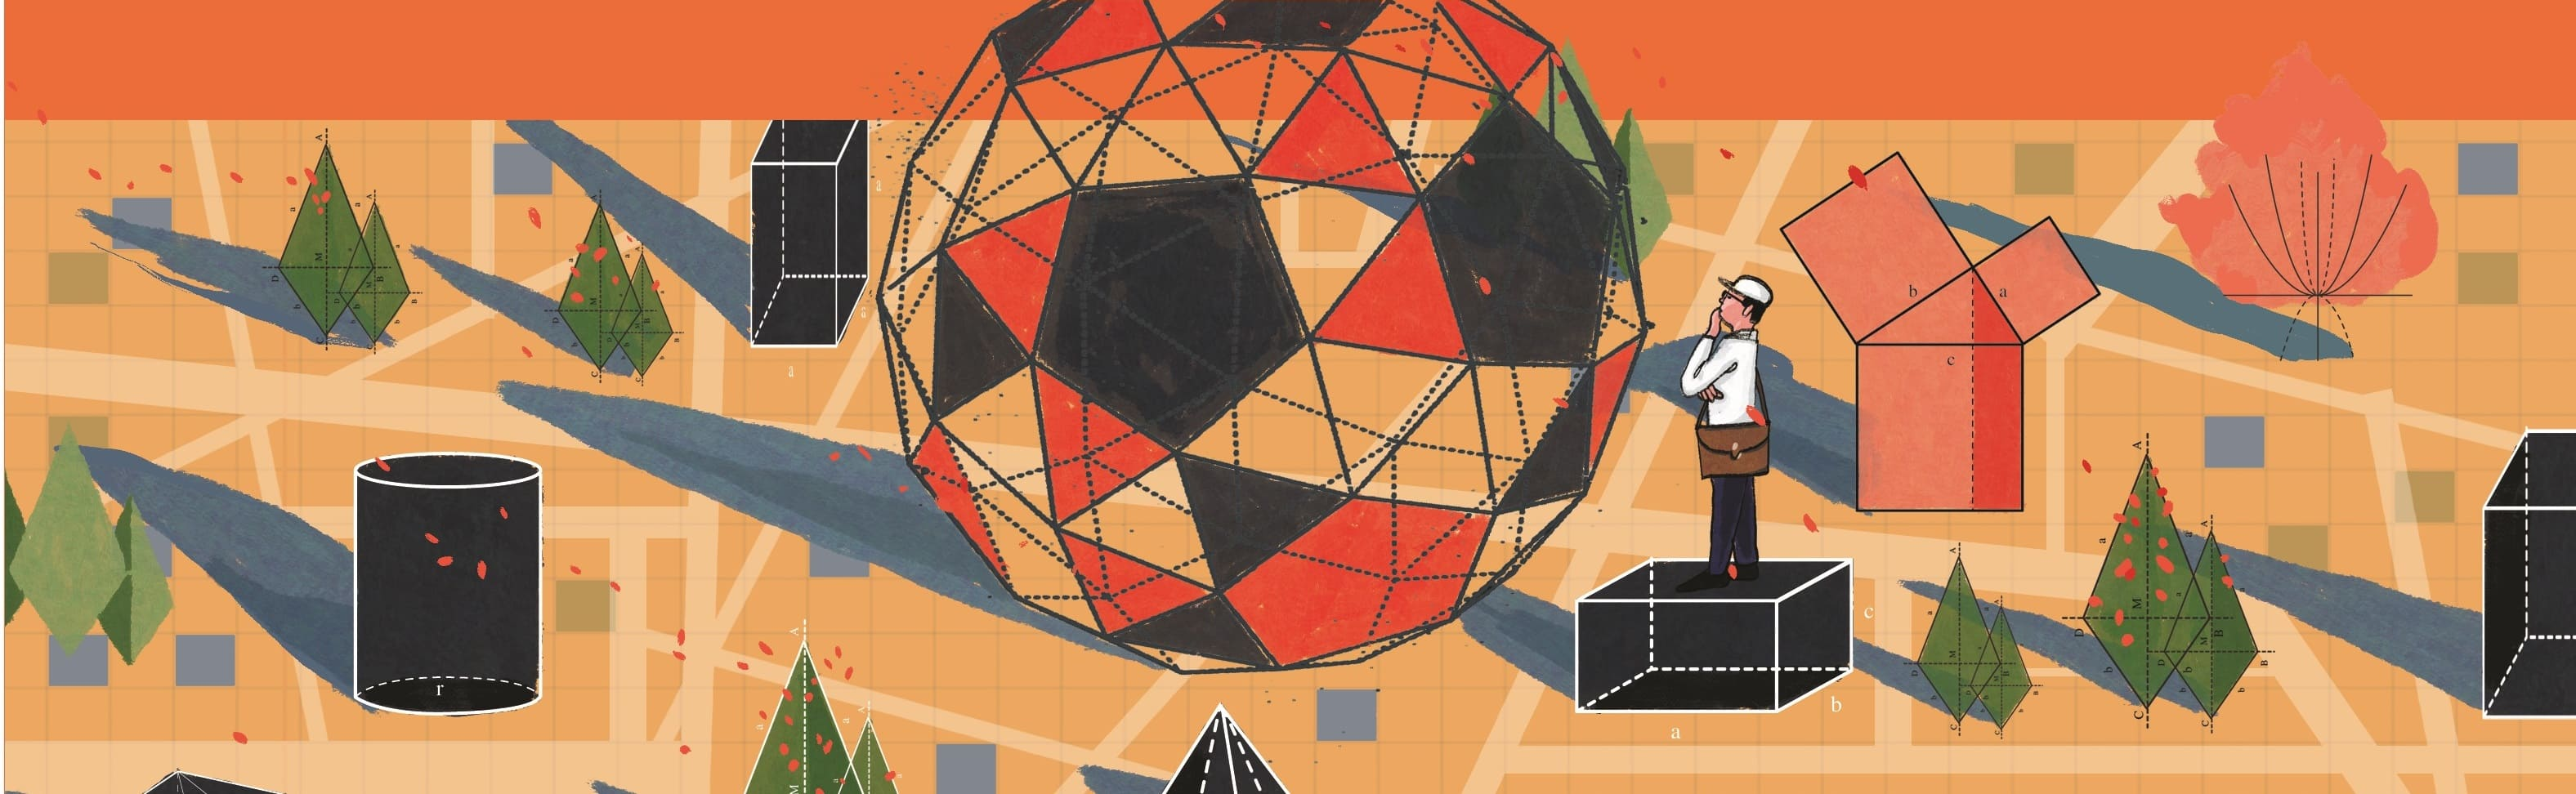
\includegraphics[width=19.3cm]{../bannerduongvao}}}
\AddToShipoutPicture*{\put(78,476){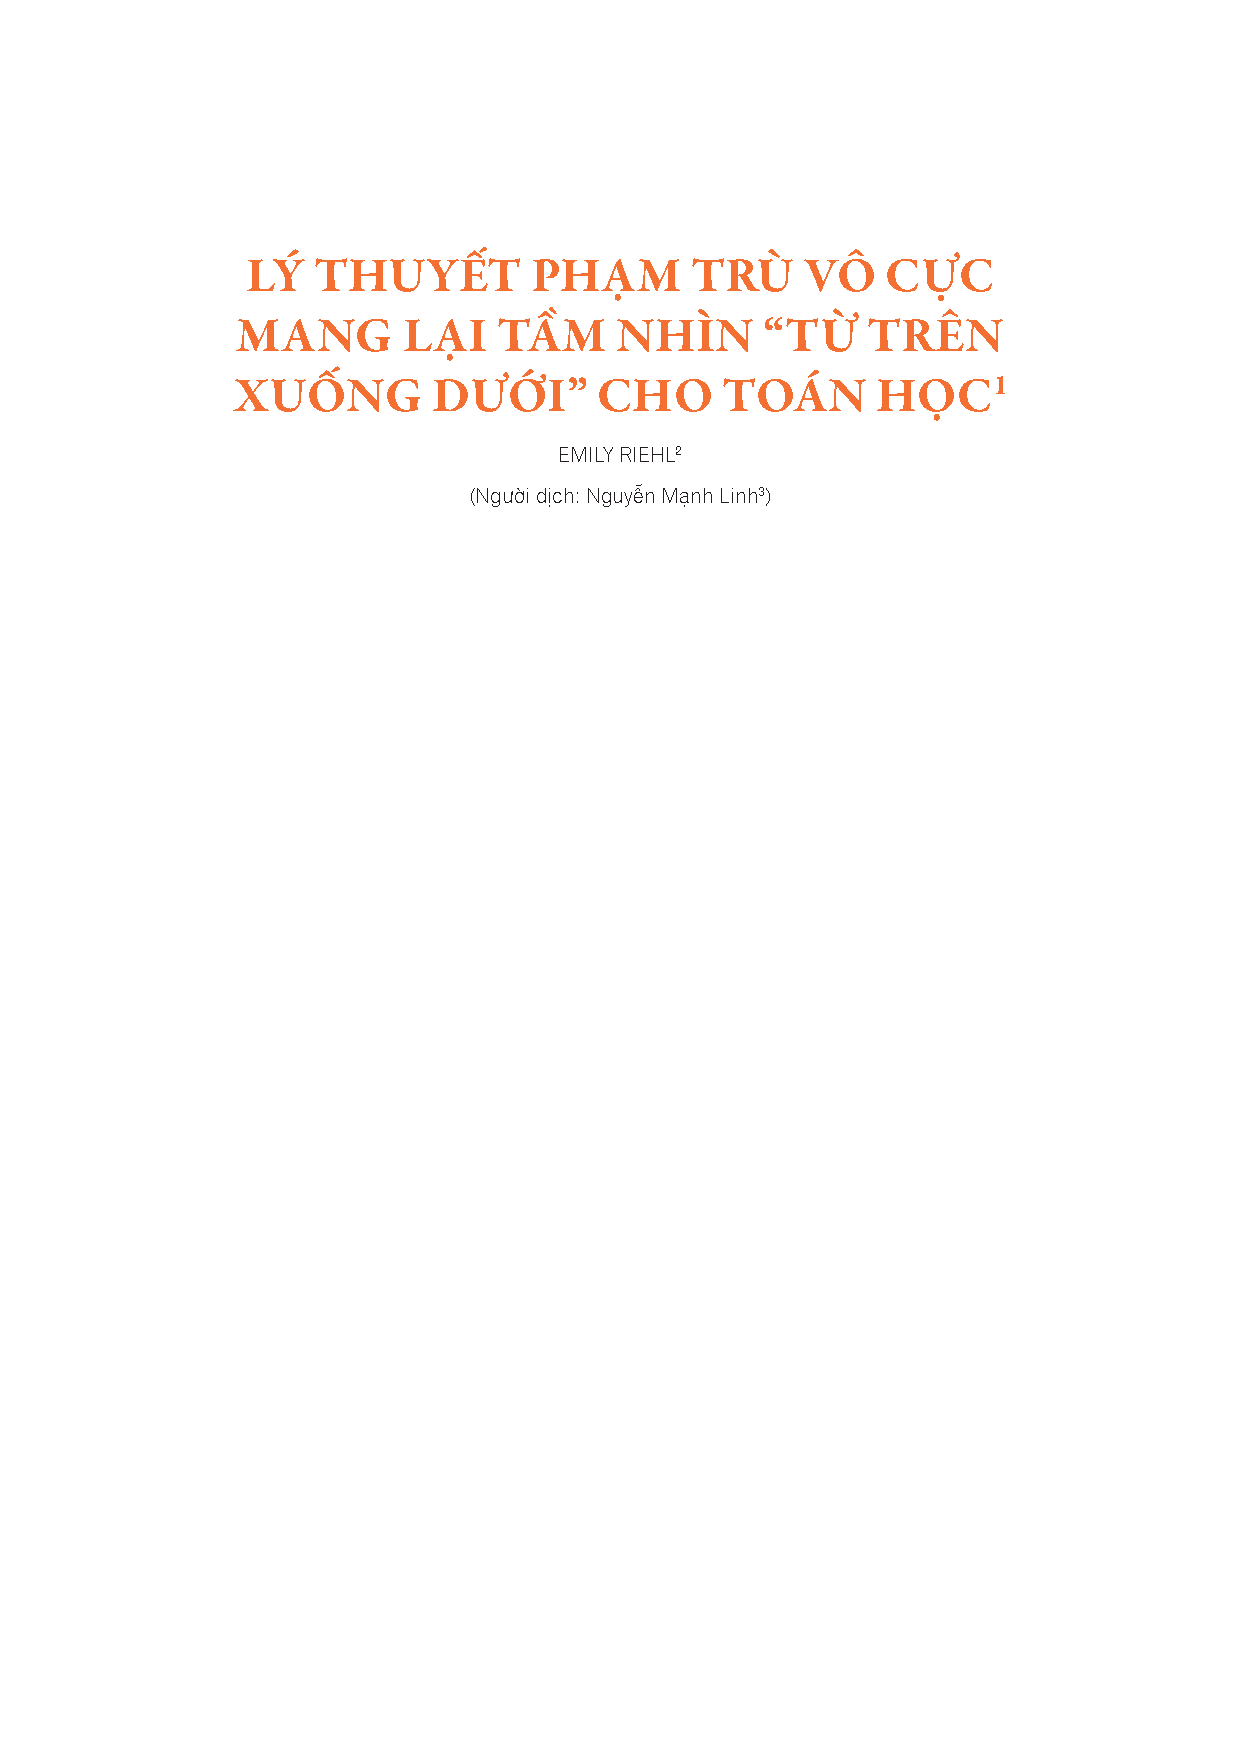
\includegraphics[scale=1]{../tieude1.pdf}}}
\centering
\endgroup

\vspace*{228pt}

\begin{multicols}{2}	
	Một ngày thu ở New England, khi còn là sinh viên năm ba, tôi đi ngang qua một ga tàu điện ngầm và một bài toán đã lọt vào mắt tôi. Một người đàn ông cùng những ý tưởng được vẽ nguệch ngoạc trên tường, một trong số đó là bài toán dựng một hình lập phương với thể tích gấp đôi một hình lập phương khác cho trước, bằng thước thẳng và compa. 
	\vskip 0.1cm
	Điều này làm tôi phải dừng lại. Tôi đã thấy bài toán này trước đây, đó là một câu đố từ hơn hai thiên thiên kỷ trước, mà theo Plutarch thì tác giả là Plato. Một thanh thước thẳng (lý tưởng) cho phép kéo dài một đoạn thẳng theo cả hai hướng, và một chiếc compa cho phép vẽ một đường tròn với bán kính tùy ý và tâm cho trước. Cái khó của câu đố này là các điểm và độ dài được dựng ra sau cùng hoặc phải có từ đầu, hoặc phải được dựng từ những thông tin trước đó.
	\vskip 0.1cm
	Để gấp đôi thể tích của hình lập phương, ta bắt đầu với độ dài cạnh của nó. Ta hoàn toàn có thể xem độ dài này là $1$ vì đó là độ dài duy nhất được cho trước. Để dựng hình lập phương lớn, ta cần tìm cách dựng cạnh của nó với độ dài yêu cầu, ở đây là $\sqrt[3]{2}$, mà chỉ dùng thước thẳng và compa.
	\vskip 0.1cm
	Đây là một bài toán khó. Không ai giải được nó sau hơn $2000$ năm. Cuối cùng thì, vào năm $1837$, Pierre Laurent Wantzel đã giải thích tại sao chưa ai thành công, bằng cách chứng minh rằng bài toán không có lời giải. Chứng minh của ông sử dụng thứ toán học tối tân bấy giờ, được đặt nền móng bởi nhà toán học Pháp đương đại \'Evariste Galois, người đã chết ở tuổi $20$ trong một cuộc đấu súng mà có lẽ là vì một drama ngoại tình. Cũng ở tuổi $20$, bản thân tôi không đạt được những thành tựu toán học ấn tượng như vậy, nhưng ít nhất tôi cũng hiểu được chứng minh của Wantzel.
	\vskip 0.1cm
	Ý tưởng như sau: Cho trước một điểm làm gốc và một đoạn với độ dài $1$, ta dễ dàng dựng được tất cả các điểm trên trục số với tọa độ hữu tỷ (tất nhiên ta đã lờ đi, như các nhà toán học hay làm, sự thật rằng ta không thể vẽ vô hạn điểm trong thời gian hữu hạn).
	\vskip 0.1cm
	Wantzel đã chứng minh rằng, chỉ bằng những công cụ trên, mỗi điểm mới dựng phải là nghiệm của một phương trình đa thức bậc hai $ax^2 + bx + c = 0$ với các hệ số $a, b, c$ thu được từ các điểm đã dựng trước đó. Tuy nhiên, điểm $\sqrt[3]{2}$ lại là nghiệm của phương trình đa thức bậc ba $x^3 - 2 = 0$, và lý thuyết ``mở rộng trường" của Galois đã chứng minh một cách thuyết phục rằng bạn không thể thu được nghiệm của một đa thức bất khả quy bậc ba chỉ bằng cách giải các phương trình bậc hai, về cơ bản là vì $3$ không phải là lũy thừa của $2$.
	\begin{figure}[H]
		\centering
		\vspace*{-5pt}
		\captionsetup{labelformat= empty, justification=centering}
		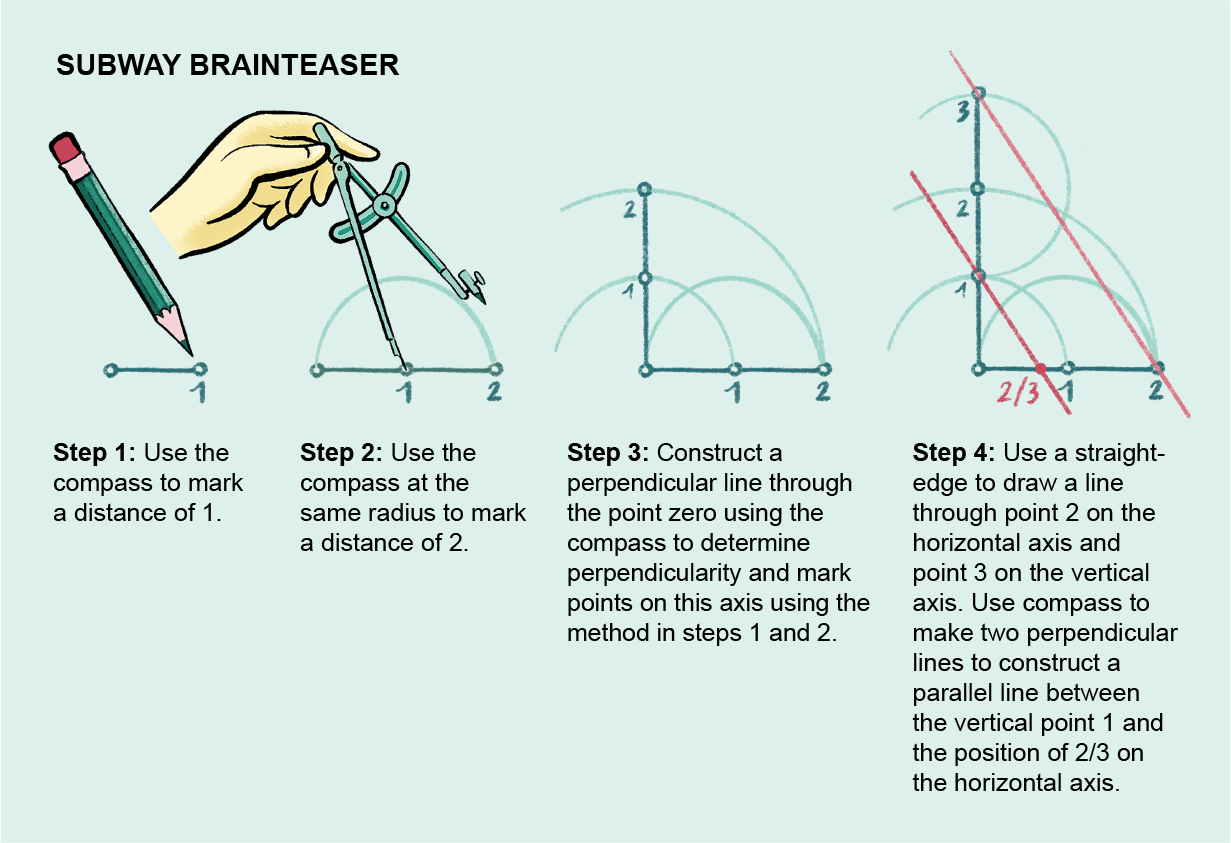
\includegraphics[width=1\linewidth]{1}
		\caption{\small\textit{\color{duongvaotoanhoc}Thước thẳng và compa cho phép dựng mọi số hữu tỷ.}}
		\vspace*{-10pt}
	\end{figure}
	Với ``vũ khí đầy mình'', tôi không kìm được mà lại gần người đàn ông trên đường. Đúng như dự đoán, nỗ lực giải thích, rằng vì sao tôi biết bài toán này không có lời giải, đã không đi tới đâu cả. Ngược lại, người đàn ông tuyên bố rằng những gì được dạy đã khiến tôi trở nên bảo thủ và không thể ``mở mang cái đầu ra''. Sau cùng, bạn gái đã kéo được tôi khỏi cuộc tranh cãi và chúng tôi tiếp tục đi.
	\vskip 0.1cm
	Nhưng vẫn còn đó một câu hỏi thú vị: Tại sao tôi, một đứa sinh viên năm ba vắt mũi chưa sạch, lại có thể học được cách dễ dàng thao túng các hệ thống số trừu tượng như các trường Galois chỉ trong vài tuần? Phần cuối của lớp học đó gồm nhóm đối xứng, vành đa thức và các cấu trúc liên quan, những thứ có lẽ sẽ làm đau đầu cả những người khổng lồ như Isaac Newton, Gottfried Leibniz, Leonhard Euler hay Carl Friedrich Gauss. Tại sao các nhà toán học lại có thể dạy cho các thế hệ sinh viên sau những khám phá làm kinh động cả những chuyên gia ở thế hệ trước?
	\begin{figure}[H]
		\centering
		\vspace*{-5pt}
		\captionsetup{labelformat= empty, justification=centering}
		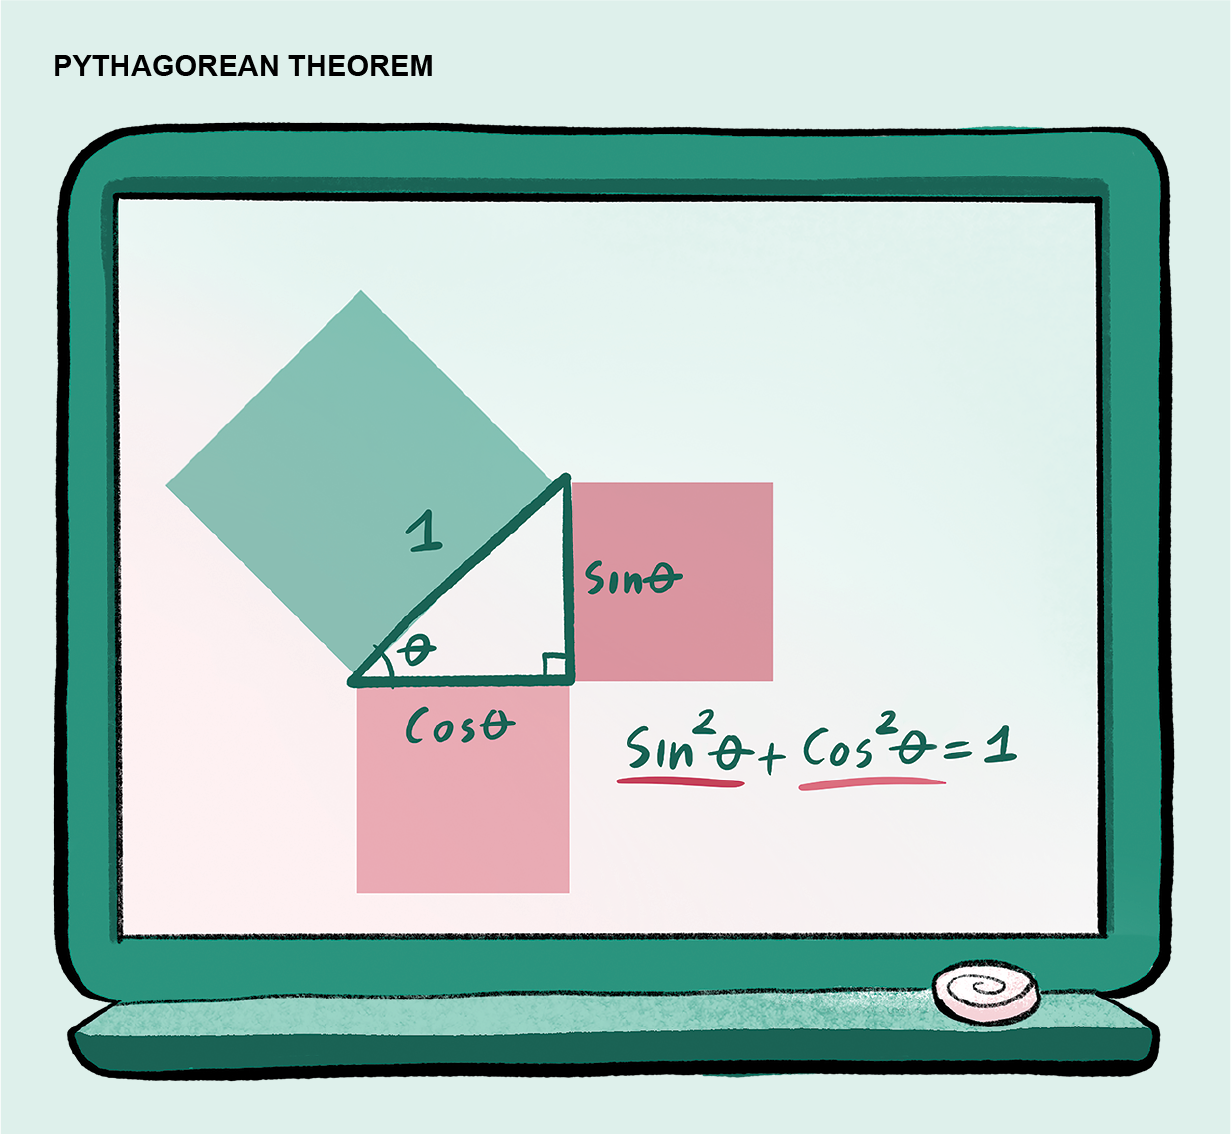
\includegraphics[width=1\linewidth]{2}
		\caption{\small\textit{\color{duongvaotoanhoc}Đẳng thức $\sin^2\theta + \cos^2\theta = 1$ từ định lý Pythagore.}}
		\vspace*{-10pt}
	\end{figure}
	Một phần câu trả lời đến từ những tiến bộ gần đây của toán học, thứ mang lại một cái nhìn ``từ trên xuống'', thông qua các cấp độ trừu tượng ngày càng tăng. Lý thuyết phạm trù là một nhánh toán học giải thích khi nào những đối tượng toán học khác nhau được coi là ``như nhau''. Định lý cơ bản của nó nói rằng bất kỳ đối tượng nào, bất kể phức tạp ra sao, đều hoàn toàn xác định khi biết quan hệ của nó với các đối tượng tương tự. Nhờ lý thuyết phạm trù, chúng ta dạy các nhà toán học trẻ những ý tưởng mới nhất bằng những quy tắc tổng quát có thể áp dụng cho những phạm trù khác nhau của toán học, thay vì đào sâu vào những quy luật đặc trưng chỉ áp dụng được trong một lĩnh vực đơn lẻ.
	\vskip 0.1cm
	Khi toán học liên tục tiến hóa, cảm nhận của các nhà toán học về sự ``như nhau'' của hai vật cũng mở rộng theo. Trong vài thập kỷ vừa qua, tôi cùng nhiều nhà nghiên cứu đang phát triển lý thuyết phạm trù để hợp lý hóa khái niệm ``duy nhất'' mới này. Những phạm trù mới, gọi là phạm trù vô cực ($\infty$--phạm trù), đã mở rộng lý thuyết phạm trù lên vô hạn chiều. Ngôn ngữ $\infty$--phạm trù mang lại cho các nhà toán học những công cụ mạnh mẽ để nghiên cứu những bài toán mà quan hệ giữa các vật quá rắc rối để có thể định nghĩa bằng phạm trù cổ điển. Góc nhìn ``thu nhỏ đến vô hạn'' này mang lại một cách nghĩ mới mẻ cho những khái niệm cũ cũng như một con đường để khám phá những khái niệm mới.
	\vskip 0.1cm
	\textbf{\color{duongvaotoanhoc}Phạm trù}
	\vskip 0.1cm
	Giống như nhiều đồng nghiệp của mình, tôi bị toán học lôi cuốn phần vì trí nhớ tệ của mình. Điều này có thể làm nhiều người bối rối khi họ nhớ rằng môn toán ở phổ thông là một mớ công thức phải thuộc -- các đẳng thức lượng giác chẳng hạn. Nhưng tôi lại thấy chúng rất dễ chịu vì hầu hết những công thức thường dùy đều có thể rút ra từ $\sin^2 \theta + \cos^2 \theta = 1$, đẳng thức mà tự thân nó có một kiến giải hình học tao nhã: đó chỉ là hệ quả trực tiếp của định lý Pythagore cho tam giác vuông với cạnh huyền bằng $1$ và một góc nhọn bằng $\theta$.
	\vskip 0.1cm
	Viễn cảnh toán học lý tưởng này, nơi mà mọi thứ đều ``hợp lý'' và chẳng cần ghi nhớ gì hết, đã phần nào đó sụp đổ ở cấp đại học. Lúc này, sinh viên được biến đến một rổ đối tượng toán học được triệu hồi từ vài thế kỷ trước. ``Nhóm'', ``vành'' và ``trường'' thuộc về lĩnh vực toán học được gọi là Đại số, một từ có nguồn gốc từ cuốn sách viết ở thế kỷ IX bởi nhà toán học, thiên văn học Ba Tư Muhammad ibn Musa al--Khwarizmi, mà tựa sách dịch ra đại khái là "Khoa học của phục hồi và cân bằng". Suốt thiên niên kỷ sau đó, đại số đã tiến hóa từ việc nghiên cứu bản chất nghiệm của các hệ phương trình đa thức thành nghiên cứu các hệ thống số trừu tượng. Vì không có số thực $x$ nào thỏa mãn phương trình $x^2+1 = 0$, các nhà toán học đã tạo ra một hệ thống số mới -- mà ngày nay gọi là số phức -- bằng cách thêm một số ảo $i$ và quy định rằng $i^2+1 = 0$.
	\vskip 0.1cm
	Đại số chỉ là một trong nhiều môn học ở chương trình toán đại học. Những môn cơ bản khác gồm Tôpô học -- nghiên cứu trừu tượng về các không gian -- và Giải tích, môn học bắt đầu với việc chặt chẽ hóa các tính toán trên hàm thực, trước khi rẽ sang những miền đất xa lạ hơn như không gian xác suất, biến ngẫu nhiên, đa tạp phức hay hàm chỉnh hình. Làm sao để sinh viên có thể thấy tất cả chúng đều hợp lý?
	\begin{figure}[H]
		\centering
		\vspace*{-5pt}
		\captionsetup{labelformat= empty, justification=centering}
		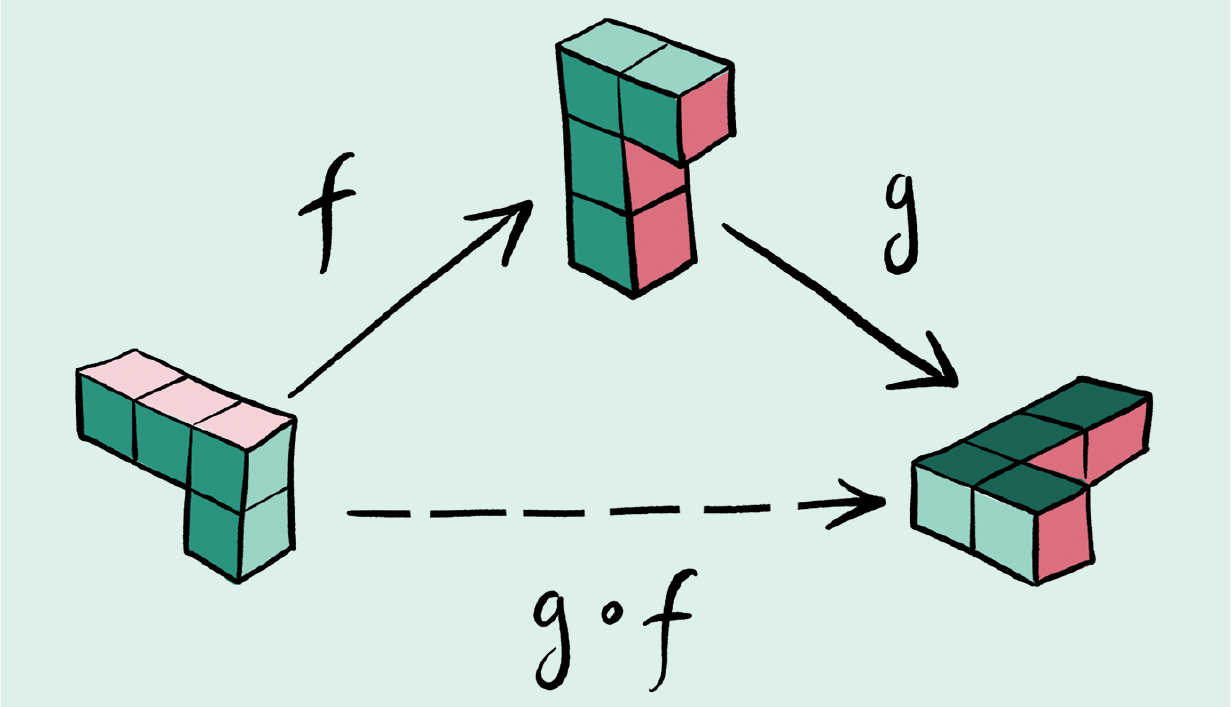
\includegraphics[width=1\linewidth]{3}
		\caption{\small\textit{\color{duongvaotoanhoc}Hợp thành của hai phép biến đổi là một phép biến đổi mới.}}
		\vspace*{-10pt}
	\end{figure}
	Một ý tưởng toán học nghe có vẻ mâu thuẫn là đơn giản hóa bằng cách trừu tượng hóa. Như Eugenia Cheng đã viết trong ``The Art of Logic in an Illogical World'' (Nghệ thuật của logic trong một thế giới phi logic), ``một trong những sức mạnh của trừu tượng hóa là nhiều bối cảnh khác nhau trở nên giống nhau khi bạn quên đi một số chi tiết.'' Đại số hiện đại được tạo ra đầu thế kỷ XX khi các nhà toán học quyết định thống nhất nghiên cứu của họ trên nhiều ví dụ khác nhau về các cấu trúc đại số xuất hiện khi xem xét nghiệm của các hệ phương trình đa thức hay các cấu hình trong mặt phẳng. Để liên kết việc tìm hiểu các cấu trúc này, họ xác định các ``tiên đề'' mô tả những tính chất chung của chúng. Nhóm, vành và trường đã được đưa vào thế giới toán học, cùng ý tưởng rằng một đối tượng toán học có thể được mô tả bằng những tính chất nó có và được khám phá một cách ``trừu tượng'', không phụ thuộc vào bối cảnh của những ví dụ hay xây dựng cụ thể.
	\vskip 0.1cm
	John Horton Conway đã có một suy nghĩ nổi tiếng về bản thể luận kỳ lạ của các sự vật toán học: ``Chúng chắc chắn có tồn tại, nhưng bạn không thể động chạm gì mà chỉ có thể nghĩ về chúng. Điều này thật đáng kinh ngạc, và tôi vẫn chưa hiểu, dù đã là nhà toán học suốt cuộc đời mình. Rằng làm thế nào một sự vật có thể ở đó mà lại không thực sự ở đó?''
	\begin{figure}[H]
		\centering
		\vspace*{-5pt}
		\captionsetup{labelformat= empty, justification=centering}
		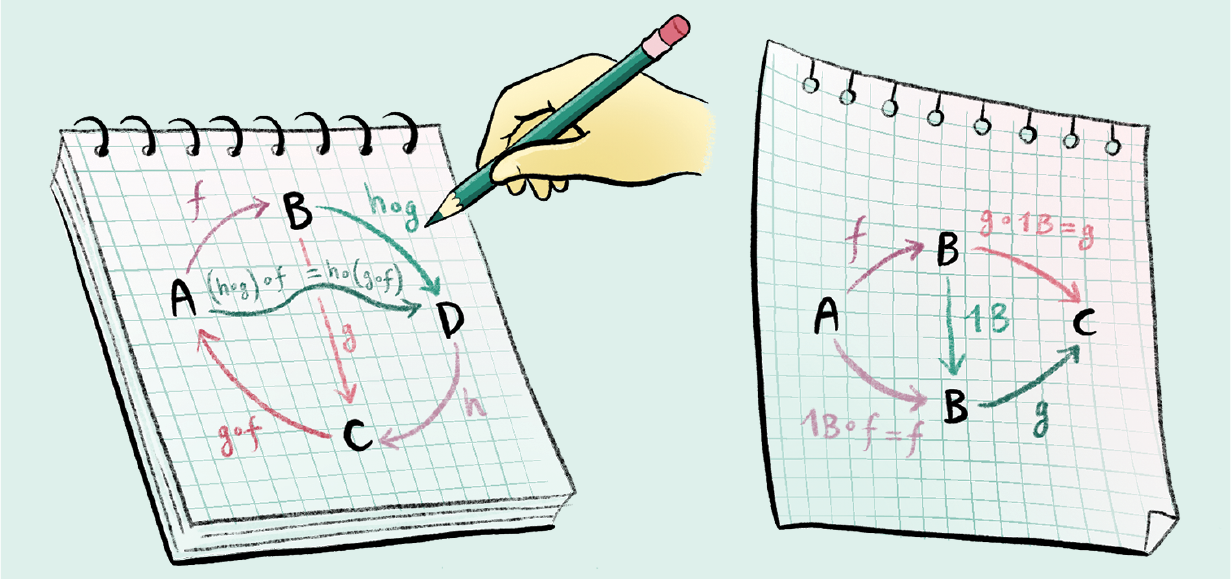
\includegraphics[width=1\linewidth]{4}
		\caption{\small\textit{\color{duongvaotoanhoc}Phép hợp thành có tính kết hợp và có đơn vị.}}
		\vspace*{-10pt}
	\end{figure}
	Nhưng thế giới của các đối tượng toán học tồn--tại--mà--không--thực--sự--ở--đó này có một vấn đề: Nó quá lớn cho bất kỳ ai để có thể hiểu được. Ngay trong đại số thôi đã có quá nhiều sự vật toán học để nghiên cứu, nhưng lại có quá ít thời gian để thể có thể thấy thấy cả đều hợp lý. Vào khoảng thế kỷ XX, các nhà toán học bắt đầu nghiên cứu đại số phổ dụng,  gồm một ``tập hợp'', có thể là một họ những phép đối xứng, những con số trong một hệ thống hoặc thứ gì đó hoàn toàn khác, cùng một số phép toán -- chẳng hạn như phép cộng và phép nhân -- thỏa mãn một loạt các tiên đề liên quan như tính kết hợp, tính giao hoán hay tính phân phối. Với những điều chỉnh khác nhau như: ``Phép toán được định nghĩa cục bộ hay toàn cục?'', ``Nó có khả nghịch không?'', người ta thu được những cấu trúc đại số cơ bản: nhóm, vành và trường. Nhưng toán học thì không bị hạn chế bởi những điều chỉnh này, điều này cho thấy một phần rất nhỏ so với số lượng vô hạn các khả năng có thể xảy ra.
	\vskip 0.1cm
	Sự sinh sôi của các đối tượng toán học trừu tượng mới mang lại sự phức tạp cho chính chúng. Một cách để đơn giản hóa là trừu tượng hóa hơn nữa, đến mức ta có thể chứng minh các định lý cho hàng loạt đối tượng cùng lúc mà không cần biết rằng cụ thể chúng ta nói về loại đối tượng nào.
	\vskip 0.1cm
	Lý thuyết phạm trù, ra đời vào những năm $40$ bởi Samuel Eilenberg và Saunders Mac Lane, đã làm chính việc này. Dù ban đầu nó được đưa ra để định nghĩa chặt chẽ thuật ngữ lỏng lẻo hay dùng là ``tương đương tự nhiên'', nó còn mang lại một cách nghĩ phổ quát về đại số phổ dụng cũng như các ngành toán học khác. Với ngôn ngữ cua Eilenberg và Mac Lane, ngày nay ta hiểu rằng mỗi loại đối tượng toán học đều thuộc về một phạm trù riêng, được định nghĩa là một họ các ``vật'' cùng các phép biến đổi được vẽ dưới dạng ``mũi tên'' giữa các vật. Chẳng hạn, trong đại số tuyến tính, người ta nghiên cứu các không gian véc tơ trừu tượng như không gian Euclid $3$--chiều. Các phép biến đổi tương ứng được gọi là các biến đổi tuyến tính, và mỗi phép biến đổi phải có một không gian nguồn và một không gian đích (đầu vào và đầu ra của phép biến đổi). Cũng như các hàm số, các phép biến đổi trong một phạm trù có thể ``hợp thành'' với nhau, nghĩa là ta áp dụng một phép biến đổi lên kết quả một phép biến đổi khác. Cho một cặp phép biến đổi $f: A \to B$ (đọc là ``$f$ là một phép biến đổi từ $A$ vào $B$'') và $g: B \to C$, quy tắc của phạm trù trả về một phép biến đổi hợp thành duy nhất, ký hiệu bởi $g \circ f: A \to C$ (đọc là ``$g$ hợp $f$ là một phép biến đổi từ $A$ vào $C$''). Cuối cùng, quy tắc hợp thành này có tính kết hợp, nghĩa là $h \circ (g \circ f) = (h \circ g) \circ f$. Nó cũng có đơn vị: mỗi vật $B$ đều có một ``biến đổi đồng nhất", thường ký hiệu bởi $\pmb{1}_B$, thỏa mãn tính chất $g \!\circ\! \pmb{1}_B \!=\! g$ và $\pmb{1}_B \!\circ\! f \!=\! f$ với mọi phép biến đổi $g$ và $f$ lần lượt có nguồn và đích là $B$. 
	\vskip 0.1cm
	Làm thế nào mà các phạm trù có thể giúp cô hay cậu sinh viên bất hạnh, người đã phải gặp quá nhiều đối tượng toán học và chẳng có đủ thời gian học hết? Bất kỳ lớp cấu trúc nào trong đại số phổ dụng có thể khác các lớp khác, nhưng các phạm trù chứa chúng thì rất giống nhau, theo một cách có thể diễn tả chính xác bằng ngôn ngữ phạm trù.
	\vskip 0.1cm
	Với đủ kinh nghiệm, một nhà toán học sẽ biết rằng họ sẽ thấy gì khi gặp một kiểu đổi tượng đại số mới. Ý tưởng này được thể hiện trong các sách toán hiện đại mà lý thuyết nhóm, vành và không gian véctơ được trình bày theo một chuỗi, về cơ bản là các lý thuyết đó song song với nhau. Có những sự tương tự khác, lỏng lẻo hơn, giữa những những phạm trù này và một số phạm trù mà sinh viên gặp trong các môn tôpô hay giải tích, và những sự tương đồng đó đó giúp họ tiếp thu tài liệu mới nhanh hơn. Những khuôn mẫu như vậy cho phép sinh viên có thêm thời gian khám phá các chủ đề cụ thể có vai trò phân biệt các lĩnh vực của toán học -- mặc dù những tiến bộ trong nghiên cứu toán học thường đến từ những sự tương tự mới và đáng ngạc nhiên giữa hai lĩnh vực không liên quan trước đó.
	\vskip 0.1cm
	\textbf{\color{duongvaotoanhoc}Đối xứng}
	\vskip 0.1cm
	Các tầng trừu tượng, từ những cấu trúc toán học cụ thể đến những hệ tiên đề và sau đó là các vật trong phạm trù, mở ra một thách thức mới: sự ``như nhau'' giữa một vật và một vật khác không còn rõ ràng nữa. Chẳng hạn, một nhóm, đối tượng toán học được cho bởi một họ trừu tượng các phép đối xứng mà các phần tử của nó được Amie Wilkinson (Đại học Chicago) mô tả như những ``chuyển động'' lật hoặc xoay một đối tượng để đưa nó về trạng thái gần giống như ban đầu.
	\vskip 0.1cm
	Chẳng hạn, ta có thể khám phá các phép đối xứng của một chiếc áo thun. Có một phép đối xứng được coi là ``chuyển động đồng nhất'', khi mà người mặc chỉ đơn thuần là giữ chiếc áo thun như bình thường. Một phép đối xứng khác ứng với chuyển động mà người mặc bỏ tay ra khỏi tay áo, giữ áo ở cổ, xoay áo $180$ độ và cho tay vào tay áo đối diện: mặt phải của áo vẫn ở ngoài nhưng áo được mặc ngược ra sau. Một phép đối xứng khác nữa ứng với chuyển động mà người mặc cởi áo ra, lộn mặt trong ra ngoài và mặc lại sao cho mỗi tay ở đúng tay áo ban đầu.  Lúc này chiếc áo thun bị lộn ngược trong ra ngoài và sau ra trước. Một phép đối xứng cuối cùng là kết hợp hai chuyển động trên: không giống như với phần lớn các nhóm, hai chuyển động này có thể thực hiện theo thứ tự tùy ý mà không làm thay đổi kết quả. Mỗi một trong bốn chuyển động trên được coi là một phép đối xứng vì sau cùng chiếc áo thun được mặc nói chung là giống như lúc đầu.
	\begin{figure}[H]
		\centering
		\vspace*{-5pt}
		\captionsetup{labelformat= empty, justification=centering}
		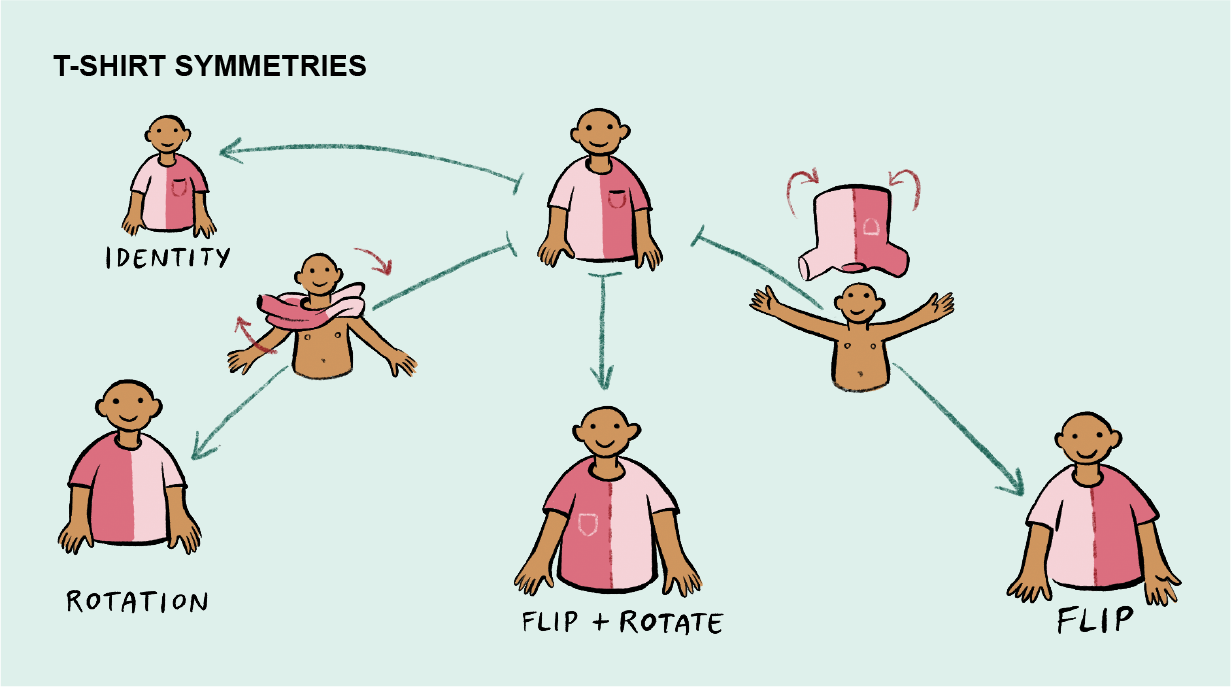
\includegraphics[width=1\linewidth]{5}
		\caption{\small\textit{\color{duongvaotoanhoc}Các phép đối xứng trên áo thun.}}
		\vspace*{-10pt}
	\end{figure}
	Một nhóm khác là ``nhóm lật thảm'', nó mô tả các đối xứng của một tấm thảm. Bên cạnh chuyển động đồng nhất (tức là giữ nguyên tấm thảm), ta có thể xoay nó $180$ độ, hoặc lật mặt dưới lên trên, hoặc kết hợp cả hai (tấm thảm nói chung không phải là hình vuông, nhưng nếu nó là hình vuông thì ta sẽ có nhiều phép đối xứng hơn nữa). Dù chiếc áo thun chẳng liên quan gì đến tấm thảm, có một trực giác rằng hai nhóm đối xứng trên có cùng ``dạng'' với nhau. Thứ nhất, cả hai nhóm đều có cùng số chuyển động (ở đây là bốn) và quan trọng hơn là ta có thể ghép mỗi chuyển động ở nhóm áo thun với nhóm lật thảm sao cho phép hợp thành chuyển động ở hai nhóm tương thích với nhau. Nói cách khác, ta có thể ghép cặp các chuyển động ở hai nhóm (phép đồng nhất ghép với phép đồng nhất, phép lật ghép với phép lật, phép xoay ghép với phép xoay, và cứ như vậy). Thứ hai, nếu ta lấy hai chuyển động từ một nhóm và thực hiện chúng theo trình tự, kết quả thu được sẽ giống với kết quả khi ta thực hiện hai chuyển động tương ứng từ nhóm còn lại theo trình tự. Về mặt kỹ thuật, các nhóm này được liên kết với nhau bởi một ``đẳng cấu'' (isomorphism), thuật ngữ được tạo ra bằng cách ghép từ gốc Hy Lạp \emph{isos}, nghĩa là ``bằng'', với \emph{morphe}, nghĩa là ``dạng''.
	\vskip 0.1cm
	Ta có thể định nghĩa đẳng cấu trong bất kỳ phạm trù nào, cho phép ta chuyển khái niệm này giữa các ngữ cảnh toán học khác nhau. Một đẳng cấu giữa hai vật $A$ và $B$ trong một phạm trù được cho bởi một cặp biến đổi $f: A \to B$ và $g: B \to A$ với sao cho các phép biến đổi hợp thành $g \circ f$ và $f \circ g$ lần lượt là các biến đổi đồng nhất $\pmb{1}_A$ và $\pmb{1}_B$. Trong phạm trù các không gian tôpô, khái niệm đẳng cấu được mô tả bởi một cặp hàm liên tục nghịch đảo lẫn nhau. Chẳng hạn, có một phép biến dạng liên tục cho phép bạn biến đổi một chiếc bánh vòng (chưa nướng) thành hình dạng như tách cà phê: lỗ ở giữa chiếc bánh vòng trở thành quai cầm, và phần cốc được tạo thành bằng cách dùng ngón tay ép. (Để phép biến dạng là liên tục, bạn không được xé rách chiếc bánh, đó là lý do vì sao không nên nướng bánh trước khi làm trò này.)
	\vskip 0.1cm
	Ví dụ này dẫn đến câu đùa rằng nhà tôpô học không thể phân biệt giữa tách cà phê và chiếc bánh vòng: với tư cách là các không gian trừu tượng, hai đối tượng này giống nhau. Trên thực tế, nhiều nhà tôpô học có khả năng phân biệt còn tệ hơn thế nữa kia; đó là vì họ đã sử dụng một quy ước linh hoạt hơn nhiều để mô tả tình huống khi hai không gian là ``như nhau'', họ đồng nhất hai không gian bất kỳ mà chỉ ``tương đương đồng luân'' với nhau thôi. Thuật ngữ trên là khái niệm đẳng cấu trong một phạm trù kỳ lạ hơn, phạm trù đồng luân của các không gian. Một tương đương đồng luân là một kiểu biến dạng liên tục khác, nhưng lúc này bạn được phép dính hai điểm phân biệt với nhau. Chẳng hạn, tưởng tượng rằng bạn bắt đầu với chiếc quần jean và thu gọn chiều dài của hai ống quần đến khi bạn thu được chiếc quần lọt khe, một ``không gian'' khác mà cấu trúc tôpô về cơ bản là không đổi -- nó vẫn có hai lỗ để cho chân vào, dù hai ống quần ($2$--chiều) ban đầu đã bị rút thành hai vòng dây ($1$--chiều).
	\begin{figure}[H]
		\centering
		\vspace*{5pt}
		\captionsetup{labelformat= empty, justification=centering}
		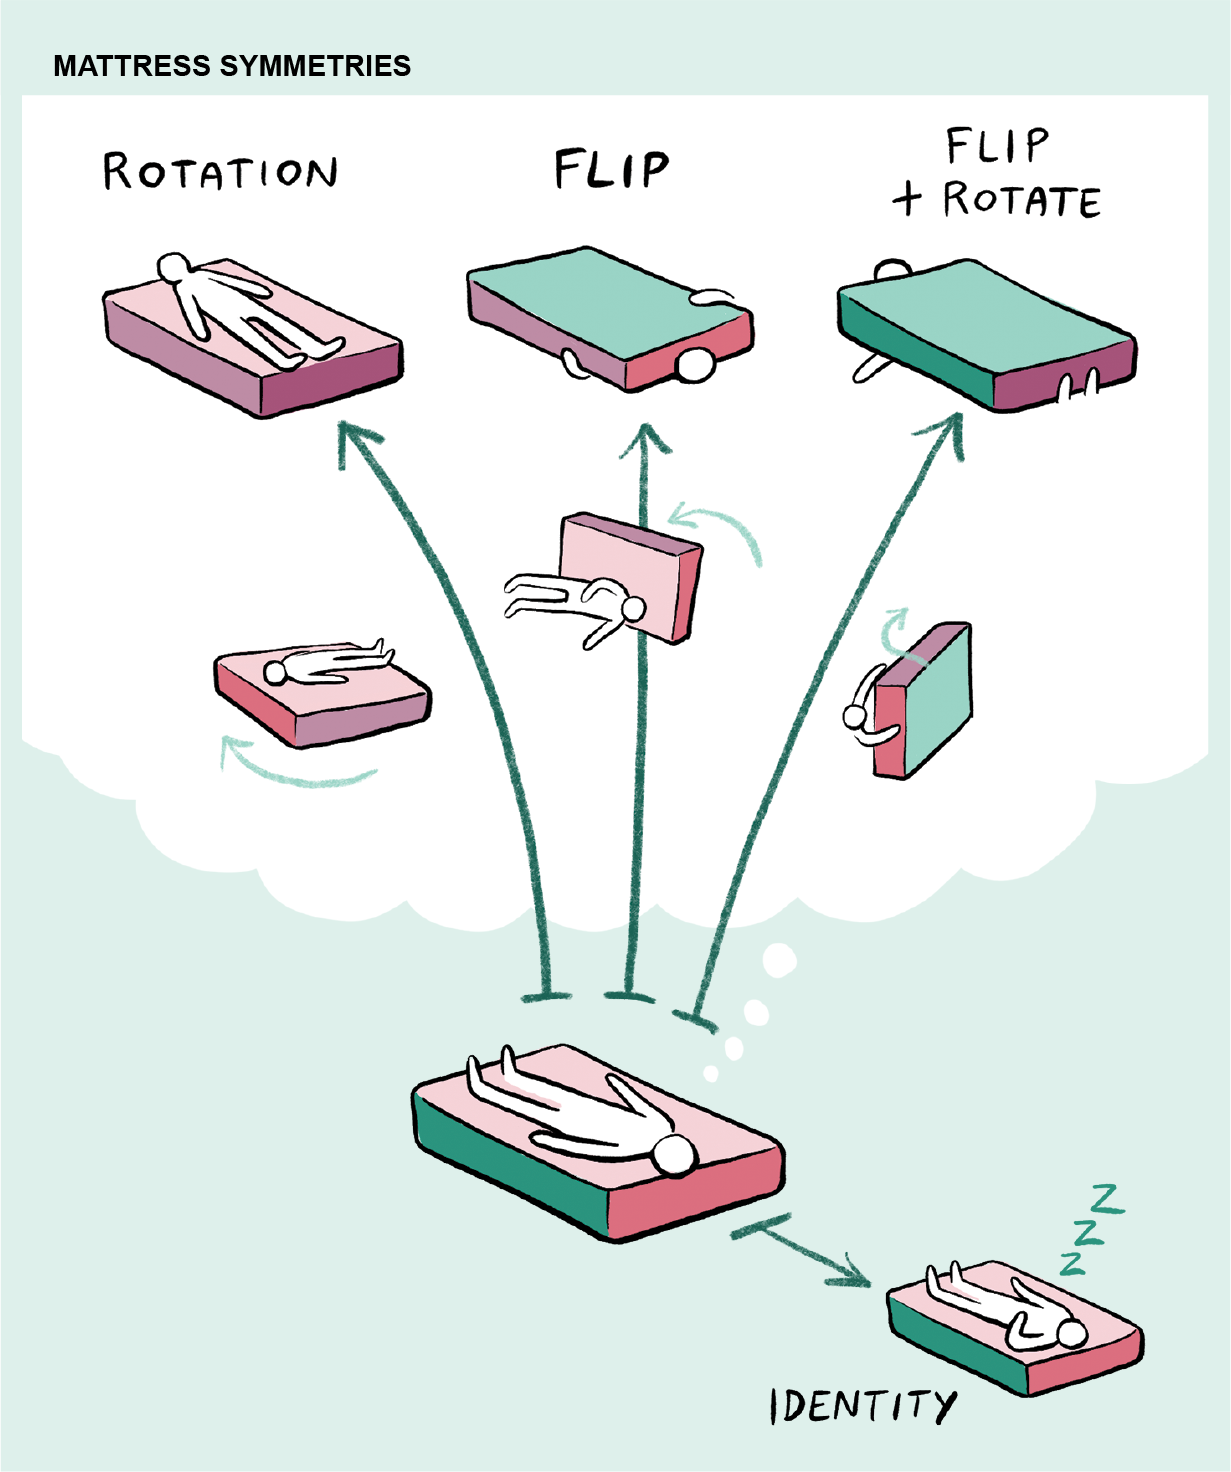
\includegraphics[width=1\linewidth]{6}
		\caption{\small\textit{\color{duongvaotoanhoc}Các phép đối xứng trên tấm thảm.}}
		\vspace*{-10pt}
	\end{figure}
	Một phép tương đương đồng luân khác thu hết toàn bộ không gian Euclid vô hạn $3$--chiều về một điểm bằng một vụ nổ ``Big Bang ngược'', khi mọi điểm đều thu về gốc, với tốc độ tăng dần theo khoảng cách giữa điểm đó với vị trí ban đầu của vụ nổ. 
	\vskip 0.1cm
	Trực giác rằng ta có thể dùng các vật đẳng cấu để thay thế nhau mà về cơ bản không làm thay đổi bản chất của phép xây dựng hay suy luận, là một trực giác rất mạnh mà các nhà lý thuyết phạm trù đã phải định nghĩa lại từ ``the'' trong tiếng Anh bởi thứ mà gần giống như từ ``$a$''. Chẳng hạn, có một khái niệm gọi là hợp rời của hai tập hợp $A$ và $B$. Giống như hợp thông thường, hợp rời $A \sqcup B$ chứa một bản sao của mỗi phần tử của $A$ cũng như của $B$. Nó khác hợp thông thường ở chỗ, nếu $A$ và $B$ có phần tử chung thì hợp rời $A \sqcup B$ chứa tới hai bản sao của phần tử đó, một bản sao ``nhớ'' rằng nó đến từ $A$ và bản sao còn lại nhớ rằng nó đến từ $B$.
	\vskip 0.1cm
	Có nhiều cách khác nhau để xây dựng hợp rời từ các tiên đề của lý thuyết tập hợp, chúng không cho chính xác cùng một tập hợp, nhưng sẽ cho các tập hợp đẳng cấu với nhau. Thay vì tốn thời gian tranh luận rằng cách xây dựng nào là chính tắc nhất, sẽ tiện hơn khi cứ giấu nhẹm sự mơ hồ này và dùng từ (the) hợp rời để chỉ bất kỳ tập hợp nào thỏa mãn bài toán phổ dụng tương ứng. Một ví dụ khác, các nhóm đối xứng áo thun và nhóm lật thảm ở trên đều được gọi là (the) nhóm bốn Klein.
	\vskip 0.1cm
	\textbf{\color{duongvaotoanhoc}Phạm trù vô cực}
	\vskip 0.1cm
	Có câu chuyện truyền miệng sau về nguồn gốc của định lý cơ bản của lý thuyết phạm trù: một nhà toán học trẻ tên Nobuo Yoneda đã mô tả một ``bổ đề'', tức là một định lý bổ trợ, cho Mac Lane ở điểm tàu Gare du Nord ở Paris năm $1954$. Yoneda bắt đầu giải thích bổ đề trên sân ga và tiếp tục ở trên tàu trước khi nó rời ga. Hệ quả của bổ đề này là mọi vật trong bất kỳ phạm trù nào đều hoàn toàn xác khi biết quan hệ của nó với các vật khác trong phạm trù đó, tức là các phép biến đổi từ vật đó vào vật khác hoặc ngược lại. Như vậy ta có thể đặc trưng một không gian tôpô $X$ bằng các nghiên cứu các hàm liên tục $f: T \to X$ đến từ các không gian $T$ khác. Chẳng hạn, một điểm trong $X$ ứng với một hàm liên tục $x: \ast \to X$ mà không gian nguồn $\ast$ là không gian với duy nhất một điểm. Ta có thể biết $X$ liên thông hay không bằng cách xét các ánh xạ $p: I \to X$ với nguồn là đoạn $I = [0,1]$. Một ánh xạ như thế là một ``đường'' có tham số trong không gian $X$ từ điểm $p(0)$ đến điểm $p(1)$, có thể xem như một quỹ đạo khả dĩ mà một con kiến có thể di chuyển trong $X$.
	\begin{figure}[H]
		\centering
		\vspace*{-5pt}
		\captionsetup{labelformat= empty, justification=centering}
		
\includegraphics[width=1\linewidth]{7}
		\caption{\small\textit{\color{duongvaotoanhoc}Các phép đối xứng trên tấm thảm.}}
		\vspace*{-10pt}
	\end{figure}	
	Ta có thể dùng các điểm và đường trong một không gian để dịch các bài toán tôpô sang đại số: Mỗi không gian tôpô $X$ có một phạm trù tương ứng $\pi_1 X$, gọi là ``phỏng nhóm cơ bản'' của $X$. Vật trong phạm trù này là các điểm của không gian, và các phép biến đổi là các đường. Nếu một đường có thể biến dạng thành một đường khác mà vẫn cố định hai đầu mút, ta quy ước rằng hai đường này định nghĩa cùng một phép biến đổi. Các biến dạng này được gọi là các phép đồng luân, ta cần chúng để mô tả phép hợp thành của đường sao cho tính kết hợp được thỏa mãn, điều kiện cần của mọi phạm trù.
	\vskip 0.1cm
	Ưu thế then chốt của phỏng nhóm cơ bản là tính ``hàm tử'', nghĩa là mọi hàm liên tục $f: X \to Y$ giữa hai không gian tôpô cho ta một phép biến đổi $\pi_1 f: \pi_1 X \to \pi_1 Y$ giữa hai phỏng nhóm cơ bản. Phép biến đổi này tôn trọng phép hợp thành và đồng nhất của đường, nghĩa là $\pi_1(g \circ f) = \pi_1 g \circ \pi_1 f$ và $\pi_1(\pmb{1}_x) = \pmb{1}_{\pi_1 x}$. Hai tính chất này, gọi chung là ``tính hàm tử'', gợi ý rằng phỏng nhóm cơ bản giữ được những tính chất cốt lõi của không gian tôpô. Nói riêng, nếu hai không gian không tương đương đồng luân thì phỏng nhóm cơ bản của chúng cũng không tương đương.
	\begin{figure}[H]
		\centering
		\vspace*{-5pt}
		\captionsetup{labelformat= empty, justification=centering}
		
\includegraphics[width=1\linewidth]{8}
		\caption{\small\textit{\color{duongvaotoanhoc}Phỏng nhóm cơ bản của đường tròn.}}
		\vspace*{-10pt}
	\end{figure}
	Dù vậy, phỏng nhóm cơ bản chưa phải là một bất biến hoàn chỉnh. Có thể dễ dàng phân biệt một đường tròn với hình tròn đặc mà đường tròn ấy bao quanh. Trong phỏng nhóm cơ bản của đường tròn, các đường giữa hai điểm cho trước, sai khác biến dạng liên tục (đồng luân), được gán với các số nguyên, chỉ số vòng mà đường này quay quanh đường tròn, với dấu $+$ hoặc $-$ chỉ chiều thuận hoặc ngược kim đồng hồ. Ngược lại, trong phỏng nhóm cơ bản của hình tròn, chỉ có duy nhất (sai khác đồng luân) một đường giữa bất kỳ cặp điểm nào. Phỏng nhóm cơ bản của phần bề mặt của quả bóng, hay một mặt cầu theo ngôn ngữ tôpô, cũng thỏa mãn chính chất này: tồn tại duy nhất, sai khác đồng luân, một đường giữa hai điểm bất kỳ.
	\vskip 0.1cm
	Vấn đề lớn với phỏng nhóm cơ bản là điểm và đường không phát hiện được cấu trúc ở chiều cao hơn của không gian, vì bản thân điểm và đoạn lần lượt là $0$--chiều và $1$--chiều. Một giải pháp là xét thêm cả các hàm liên tục từ hình tròn $2$--chiều, được gọi là các phép đồng luân, cùng với các ``đồng luân bậc cao'', được định nghĩa là các hàm liên tục hình hình cầu đặc $3$--chiều và tương tự với các hình siêu cầu $4$--, $5$--, $6$--chiều hoặc hơn.
	\begin{figure}[H]
		\centering
		\vspace*{-5pt}
		\captionsetup{labelformat= empty, justification=centering}
		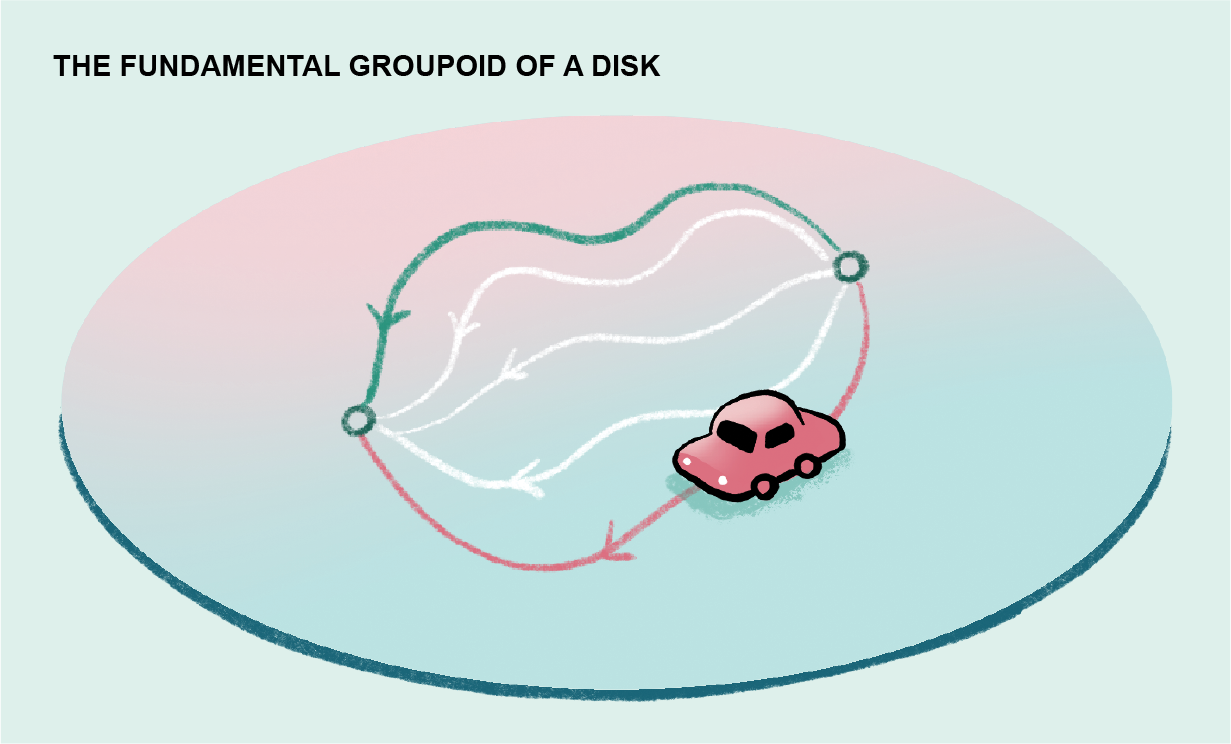
\includegraphics[width=1\linewidth]{9}
		\caption{\small\textit{\color{duongvaotoanhoc}Phỏng nhóm cơ bản của hình tròn.}}
		\vspace*{-10pt}
	\end{figure}
	Một câu hỏi tự nhiên là các điểm, đường, đồng luân và đồng luân bậc cao của một không gian $X$ thì tạo ra cấu trúc gì: cấu trúc $\pi_\infty$ này, gọi là $\infty$--phỏng nhóm cơ bản của X, định nghĩa một $\infty$--phạm trù, phiên bản vô hạn chiều của phạm trù đưa ra bởi Eilenberg và Mac Lane. Giống như phạm trù thông thường, một $\infty$--phạm trù gồm các vật và các phép biến đổi được vẽ như những mũi tên $1$--chiều, nhưng nó còn có thêm các phép ``biến đổi bậc cao'', được vẽ như các mũi tên $2$--chiều, mũi tên $3$--chiều, và cứ như vậy. Ví dụ, trong $\pi_\infty X$, các vật và các mũi tên lần lượt là các điểm và các đường -- lúc này ta không xét sai khác đồng luân nữa -- trong khi các biến đổi bậc cao lưu giữ thông tin đồng luân bậc cao. Cũng như trong phạm trù thông thường, các mũi tên (với số chiều cố định) có thể hợp thành: nếu ta có hai mũi tên $f: X \to Y$ và $g: Y \to Z$, ta phải có mũi tên thứ ba $g \circ f: X \to Z$. Nhưng cái khó ở đây là: để mô tả được những ví dụ rất tự nhiên như $\infty$--phỏng nhóm cơ bản của một không gian, luật hợp thành phải bị làm yếu đi. Với mỗi cặp mũi tên khả hợp thành, một mũi tên hợp thành tồn tại, nhưng nó không còn là duy nhất nữa.
	\vskip 0.1cm
	Sự thiếu sót của tính duy nhất này thách thức việc định nghĩa $\infty$--phạm trù bằng cơ sở toán học bởi lý thuyết tập hợp cổ điển, vì ta không thể xem phép hợp thành như một phép toán như trong đại số phổ dụng nữa. Dù $\infty$--phạm trù đang dần trở thành đối tượng trung tâm của nghiên cứu hiện đại trong nhiều lĩnh tực toán học từ lý thuyết trường lượng tử tôpô đến hình học đại số hay tôpô đại số, chúng thường được xem là ``quá khó'' cho mọi người ngoài các chuyên gia, và nó không xuất hiện thường xuyên trong chương trình học, ngay cả sau đại học. Dù vậy, tôi và nhiều người khác xem $\infty$--phạm trù như một hướng đi mới và cách mạng, cho phép các nhà toán học mơ đến những liên kết mới mà không thể phát biểu và chứng minh một cách chặt chẽ bằng cách khác.
	\vskip 0.1cm
	\centerline{\bf\color{duongvaotoanhoc}Một số thuật ngữ Toán học hiện đại}
	\vskip 0.1cm
	$\bullet$ Hợp thành: chỉ việc áp dụng một phép biến đổi lên kết quả của một phép biến đổi khác.
	\vskip 0.1cm	
	$\bullet$ Phạm trù: một họ cụ thể gồm các vật và phép biến đổi giữa chúng, cùng một luật hợp thành.
	\vskip 0.1cm	
	$\bullet$ Đồng nhất: phép biến đổi từ một vật vào chính nó mà hoàn toàn không thay đổi vật đó.
	\vskip 0.1cm			
	$\bullet$ Đối xứng: một phép biến đổi khả nghịch từ một vật vào chính nó.
	\vskip 0.1cm	
	$\bullet$ Đẳng cấu: khái niệm ``như nhau'' về mặt cấu trúc, tồn tại giữa các cặp vật trong một phạm trù.
	\vskip 0.1cm
	$\bullet$ Phỏng nhóm cơ bản: phạm trù mà vật là điểm trong một không gian và các phép biến đổi là các đường sai khác đồng luân \linebreak giữa chúng.
	\vskip 0.1cm		
	$\bullet$ Đồng luân: ``đường giữa hai đường", được định nghĩa là một biến dạng liên tục từ đường này thành đường kia.
	\vskip 0.1cm		
	$\bullet$ Phạm trù vô cực: phiên bản vô hạn chiều của phạm trù, nơi có thêm các biến đổi bậc cao và luật hợp thành bị làm yếu đi.
	\vskip 0.1cm	
	$\bullet$ Phỏng nhóm vô cực cơ bản: phạm trù vô cực gồm các điểm, đường, đồng luân và đồng luân bậc cao của một không gian.
	\vskip 0.1cm
	\textbf{\color{duongvaotoanhoc}Chân trời tương lai}
	\vskip 0.1cm
	Dẫu vậy, kinh nghiệm lịch sử cho thấy rằng phần lớn những kiến thức toán học mới lạ nhất hôm nay sẽ dần trở nên đủ dễ để dạy cho sinh viên toán ngài mai. Sẽ rất vui khi được quan sát, với tư cách là một người nghiên cứu $\infty$--phạm trù, cách mà nó có thể được đơn giản hóa đi. Chẳng hạn như một mẹo nhỏ về ngôn ngữ -- một phiên bản siêu cấp của từ ``the'' trong phạm trù -- có thể khiến cho sinh viên ở cuối thế kỷ XXI hiểu $\infty$--phạm trù một cách dễ dàng như phạm trù thông thường ngày nay. Tiên đề then chốt của lý thuyết phạm trù thông thường là sự tồn tại duy nhất của một phép biến đổi hợp thành $g \circ f: X \to Z$ với mỗi cặp biến đổi $f: X \to Y$ và $g: Y \to Z$, được chọn ra từ tập các phép biến đổi từ $X$ vào $Z$. Trái lại, trong một $\infty$--phạm trù, có một không gian các mũi tên từ $X$ vào $Z$, thứ mà trong $\infty$--phỏng nhóm cơ bản có thể hiểu là ``không gian đường''. Phiên bản đúng của tính hợp thành duy nhất trong phạm trù thông thường là mệnh đề: trong một $\infty$--phạm trù, không gian các hợp thành là ``co rút được'', nghĩa là mỗi điểm của nó đều có thể suy sụp một cách liên tục qua một vụ nổ ``Big Bang ngược'' về một điểm gốc duy nhất.
	\vskip 0.1cm
	Chú ý rằng tính co rút được không suy ra rằng có duy nhất một hợp thành: thật vậy, ta đã thấy rằng trong $\infty$--phỏng nhóm cơ bản, có thể có rất nhiều đường hợp thành. Nhưng tính co rút được đảm bảo rằng hai đường hợp thành luôn đồng luân, và hai phép đồng luân bất kỳ giữa hai đường hợp thành luôn liên kết với nhau bởi một đồng luân bậc cao, và cứ như vậy.
	\begin{figure}[H]
		\centering
		\vspace*{-5pt}
		\captionsetup{labelformat= empty, justification=centering}
		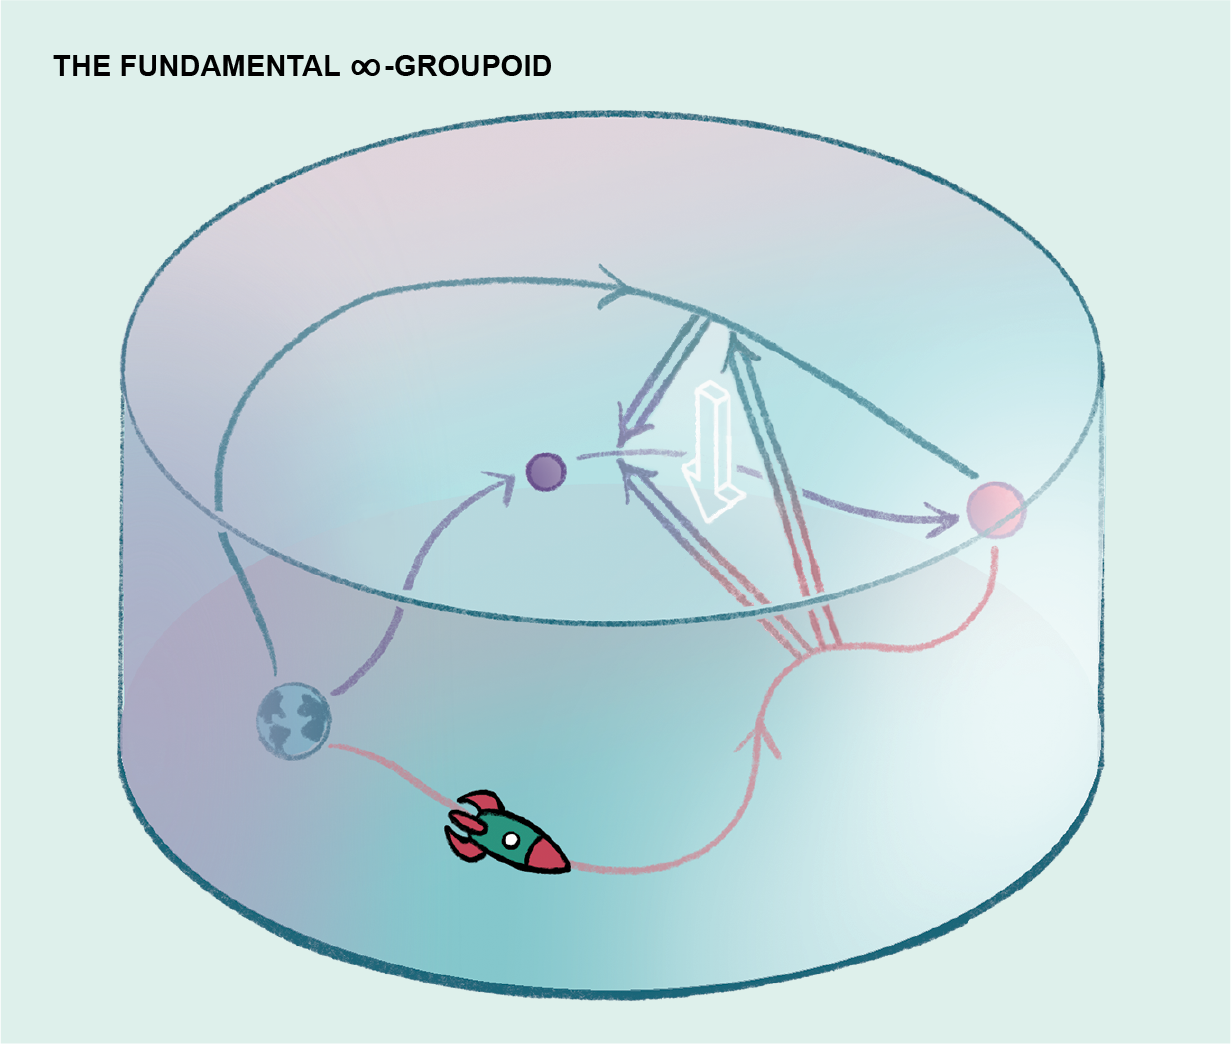
\includegraphics[width=1\linewidth]{10}
		\caption{\small\textit{\color{duongvaotoanhoc}Phỏng nhóm vô cực cơ bản.}}
		\vspace*{-10pt}
	\end{figure}
	Ý tưởng về sự duy nhất như điều kiện co rút được này là một ý tưởng trung tâm trong hệ cơ sở toán học mới được đề xuất bởi Vladimir Voedvodsky và nhiều người khác. Các nhà toán học khắp nơi đang hợp sức phát triển những ``phụ tá chứng minh'' bằng máy tính có khả năng kiểm tra từng dòng một trong chứng minh hình thức của một kết quả toán học. Những phụ tá này có một cơ chế bắt chước theo một kỹ thuật chung trong toán học là chuyển thông tin từ một vật sang một vật khác được coi là giống vật ban đầu qua một đẳng cấu tường minh hoặc một tương đương đồng luân. Cơ chế này cho phép người dùng chuyển một chứng minh liên quan đến một điểm trong không gian qua một đường nối nó đến một điểm khác, đưa ra một định nghĩa chặt chẽ về khái niệm ``như nhau'' của tôpô.
	\vskip 0.1cm
	Trong một tham luận năm $1974$, nhà toán học Micheal Atiyah đã viết ``Mục tiêu thực sự của lý thuyết là tổ chức lại một cách có hệ thống kinh nghiệm quá khứ sao cho thế hệ sau, học sinh của chúng ta, rồi học sinh của họ, rồi sau đó nữa, có thể tiếp thu những khía cạnh cốt lõi mà ít tốn sức nhất, và đó là cách duy nhất mà bạn có thể liên tục tích lũy và xây dựng bất kỳ hoạt động khoa học nào mà không đi đến ngõ cụt.'' Lý thuyết phạm trù đóng vai trò này trong toán học hiện đại: nếu toán học là khoa học của sự tương tự, các khuôn mẫu, thì lý thuyết phạm trù là khoa học của các khuôn mẫu tư duy toán học -- ``toán học của toán học'', như Eugenia Cheng (Viện Nghệ thuật Chicago), đã gọi.
	\vskip 0.1cm
	Lý do ta dạy được rất nhiều trong một môn toán ở đại học ngày nay là vì hiểu biết của chúng ta về rất nhiều khái niệm toán học khác nhau đã được đơn giản hóa nhờ sự trừu tượng, có thể xem như lùi khỏi bài toán cụ thể để quan sát tổng quan toán học. Rất nhiều chi tiết sẽ ẩn đi ở tầm này -- xấp xỉ số chẳng hạn, hoặc bất kỳ thứ gì liên quan đến số -- nhưng một sự thật đáng chú ý là nhiều định lý trong đại số, lý thuyết tập hợp, tôpô và hình học đại số thường đúng vì cùng một lý do đằng sau, và khi đó, các chứng minh được diễn tả bằng ngôn ngữ phạm trù.
	\vskip 0.1cm
	Có gì ở chân trời tương lai? Đang hình thành một sự đồng thuận trong nhiều lĩnh vực toán học rằng các đối tượng cơ bản của toán học thế kỷ XXI là các $\infty$--phạm trù, giống như ở thế kỷ XX là các phạm trù thông thường. Ta hi vọng rằng chiếc tháp vô hạn của các mũi tên ở mọi chiều này, thứ cần nghiên cứu tỷ mỉ trong $\infty$--phạm trù, đến lúc nào đó sẽ thu gọn về về tiềm thức chung của toán học, với các không gian co rút được suy sụp về một điểm duy nhất. Và ta có thể tự hỏi: Nếu những tiến bộ này xuất hiện ở thế kỷ XX, toán ở học ở cuối thế kỷ XXI sẽ đi về đâu?
\end{multicols}
\vspace*{-10pt}
{\color{duongvaotoanhoc}\rule{1\linewidth}{0.1pt}}
\begin{center}
	\textbf{\color{duongvaotoanhoc}DANH SÁCH HỌC SINH CÓ LỜI GIẢI HOÀN CHỈNH}
\end{center}
\textit{Trong các ngoặc đơn ở phần dưới đây, sau tên lớp là mã hiệu của các bài toán mà học sinh có lời giải hoàn chỉnh.}
\begin{multicols}{2}
	\textbf{\color{duongvaotoanhoc}KHỐI THCS}
	\vskip 0.05cm
	$\bullet$ Trường \textbf{\color{duongvaotoanhoc}THCS xã Pom Lót}, huyện Điện Biên, tỉnh Điện Biên: \textit{Nguyễn Ngọc Diệp} (lớp $9$D$3$; P$661$).
	\vskip 0.05cm
	\textbf{\color{duongvaotoanhoc}KHỐI THPT}
	\vskip 0.05cm
	$\bullet$ Trường \textbf{\color{duongvaotoanhoc}THPT chuyên Nguyễn Quang Diêu}, tỉnh Đồng Tháp: \textit{Lư Gia Hưng} (lớp $11$T$1$; P$662$), \textit{Đỗ Duy Quang} (lớp $11$T$1$; P$662$, P$664$).
	\vskip 0.05cm
	$\bullet$ Trường \textbf{\color{duongvaotoanhoc}THPT Chi Lăng}, tỉnh Gia Lai: \textit{Phan Trịnh Nguyên} (lớp $10$A$1$; P$661$).
	\vskip 0.05cm
	$\bullet$ Trường \textbf{\color{duongvaotoanhoc}THPT chuyên Hà Tĩnh}, tỉnh Hà Tĩnh: \textit{Trần Minh Hoàng} (lớp $10$T$1$; P$662$, P$663$, P$666$, P$667$, P$670$).
	\vskip 0.05cm
	$\bullet$ Trường \textbf{\color{duongvaotoanhoc}THPT chuyên Lê Hồng Phong}, tỉnh Nam Định: \textit{Nguyễn Hoàng Anh} (lớp $11$ Toán $2$; P$664$), \textit{Phùng Việt Cường} (lớp $11$ Toán $2$; P$661$, P$664$, P$666$), \textit{Nguyễn Đức Khải} (lớp $11$ Toán $2$; P$667$), \textit{Ninh Thị Mai Linh} (lớp $12$ Toán $1$; P$661$, P$664$), \textit{Đồng Đức Mạnh} (lớp $11$ Toán $1$; P$661$), \textit{Hà Thị Kim Oanh} (lớp $12$ Toán $1$; P$664$, P$669$), \textit{Nguyễn Xuân Tiến} (lớp $11$ Toán $2$; P$667$).
	\vskip 0.05cm
	$\bullet$ Trường \textbf{\color{duongvaotoanhoc}THPT chuyên Nguyễn Bỉnh Khiêm}, tỉnh Quảng Nam: \textit{Trịnh Quốc Khánh} (lớp $11$ chuyên Toán; P$669$).
	\vskip 0.05cm
	$\bullet$ Trường \textbf{\color{duongvaotoanhoc}THPT chuyên Tiền Giang}, tỉnh Tiền Giang: \textit{Trần Phúc Thịnh} (lớp $10$ Toán; P$661$), \textit{Nguyễn Hữu Trí} (lớp $10$ Toán; P$661$).
	\vskip 0.05cm
	$\bullet$ Trường \textbf{\color{duongvaotoanhoc}THPT chuyên Quốc học Huế}, tỉnh Thừa Thiên -- Huế: \textit{Nguyễn Thị Nhật Thảo} (lớp $11$ Toán $2$; P$661$), \textit{Trần Thị Thanh Thư} (lớp $12$ Toán $1$; P$661$), \textit{Đặng Quỳnh Bảo Uyên} (lớp $11$ Toán $2$; P$661$).
	\vskip 0.05cm
	$\bullet$ Trường \textbf{\color{duongvaotoanhoc}THPT chuyên Khoa học tự nhiên}, ĐH Khoa học tự nhiên -- ĐHQG Hà Nội: \textit{Vương Khánh Toàn} (lớp $10$A$1$ Toán; P$667$, P$668$, P$669$).
	\vskip 0.05cm
	$\bullet$ Trường \textbf{\color{duongvaotoanhoc}THPT chuyên Sư phạm}, ĐH Sư phạm Hà Nội: \textit{Hồ Trần Khánh Linh} (lớp $12$ Toán $2$; P$667$, P$669$).
\end{multicols}